% -----------------------------------------------
% Template for ISMIR Papers
% 2017 version, based on previous ISMIR templates

% Requirements :
% * 6+n page length maximum
% * 4MB maximum file size
% * Copyright note must appear in the bottom left corner of first page
% * Clearer statement about citing own work in anonymized submission
% (see conference website for additional details)
% -----------------------------------------------

% Anonymity: authors, GitHub links, acknowledgments

\documentclass{article}
\usepackage[T1]{fontenc} \usepackage[utf8]{inputenc}
\usepackage[svgnames]{xcolor}
\usepackage[bookmarks=false,colorlinks=true,allcolors=DarkBlue]{hyperref} % MidnightBlue, NavyBlue, DarkBlue, Maroon
\usepackage{ismir,amsmath}
\usepackage{graphicx} \graphicspath{{figs/}}
\usepackage{booktabs, threeparttable, tabularx}
\usepackage{enumitem} \setlist{itemsep=0pt,topsep=0pt,parsep=0pt,partopsep=0pt}

\newcommand{\todo}[1]{{\color{red} #1 }}

\title{FMA: A Dataset For Music Analysis}

\oneauthor
{Kirell Benzi, \hspace{.2cm} Michaël Defferrard, \hspace{.2cm} Pierre Vandergheynst, \hspace{.2cm} Xavier Bresson}
 {{\tt michael.defferrard@epfl.ch, kirell.benzi@epfl.ch} \\
  {\tt pierre.vandergheynst@epfl.ch, xavier.bresson@epfl.ch} \\
  LTS2, EPFL, Lausanne, Switzerland}

%\threeauthors
%  {First Author} {Affiliation1 \\ {\tt author1@ismir.edu}}
%  {Second Author} {\bf Retain these fake authors in\\\bf submission to preserve the formatting}
%  {Third Author} {Affiliation3 \\ {\tt author3@ismir.edu}}

%% To make customize author list in Creative Common license, uncomment and customize the next line
\def\authorname{Kirell Benzi, Michaël Defferrard, Pierre Vandergheynst, Xavier Bresson}

\sloppy % please retain sloppy command for improved formatting
\begin{document}
\maketitle

% about 150-200 words.
\begin{abstract}

The Free Music Archive (FMA) is an open music dataset that can be used to evaluate several tasks in music information retrieval (MIR).
The released data is composed of 110,000 tracks, xx artists, xx albums, 164 genres, for a total of 229 days of audio for 900 GiB, all under permissive Creative Commons licenses.
It features a collection of meta-data such as the song title, artist name, album or genres, together with user data such as play counts, full-length and high-quality audio, as well as a set of pre-computed features. We propose a train / test split and three subsets: a small genre-balanced dataset of 4,000 songs and 10 genres, a medium genre-unbalanced dataset of 14,511 songs and 20 genres, and a 90 GiB version of the full set, with clips trimmed to 30s.
This paper describes the dataset and how it was created, proposes some tasks and evaluate some baselines for music genre recognition (MGR).
All the code to reproduce it as well as links to download the data and usage examples are available at \url{https://github.com/mdeff/fma}.

% Our major goal is to go beyond the existing limitations of available music datasets, which are either the small size of datasets with raw audio tracks, the availability and legality of the music data, or the lack of meta-data for artists analysis or song ratings for recommender systems. Existing datasets such as GTZAN, TagATune, and Million Song suffer from the previous limitations. It is however essential to establish such benchmark datasets to advance the field of music analysis, like the ImageNet dataset which made possible the large success of deep learning techniques in computer vision.

% which contains 77,643 songs and 68 genres spanning 26.9 days of song listening
\end{abstract}



%%%%%%%%%%%%%%%%%%%%%%%%%%%%%%%%%%%%%%%%%%%%%%%%%%%%%%%%%%%%%%%%%%%%%%%%%%%%%%%%
\section{Introduction} % and Motivation}
%%%%%%%%%%%%%%%%%%%%%%%%%%%%%%%%%%%%%%%%%%%%%%%%%%%%%%%%%%%%%%%%%%%%%%%%%%%%%%%%


% hook
While the development of new mathematical models and algorithms to solve challenging real-world problems is obviously of first importance to any field of research, evaluation and comparison to the existing state-of-the-art is necessary for a technique to be widely adopted by research communities. Such tasks require benchmark datasets. % to achieve their purpose, which are sometimes challenging to collect and share.
In computer vision, the community has developed over the years established benchmark datasets such as \href{http://yann.lecun.com/exdb/mnist/}{MNIST} \cite{mnist}, \href{https://www.cs.toronto.edu/~kriz/cifar.html}{CIFAR} \cite{cifar}, or \href{http://www.image-net.org}{ImageNet} \cite{imagenet}. These datasets are free, legal, easily available, and have proved essential to advance the field. The most celebrated example, the \href{http://www.image-net.org/challenges/LSVRC/2012/}{ILSVRC2012 challenge} on an unprecedented ImageNet subset of 1.5M images, allowed to demonstrate the power of deep learning (DL), which won the competition with an 11\% accuracy advantage over the second best \cite{convnet_imagenet}.

\begin{table}[t]
	\centering
	\begin{threeparttable}
	\begin{tabular}{lrrcc}
		\toprule
		dataset & \#clips & \#artists & year & audio \\
		\midrule
		\href{https://staff.aist.go.jp/m.goto/RWC-MDB/}{RWC} \cite{RWC} & 465 & - & 2001 & yes \\
		\href{http://calab1.ucsd.edu/~datasets/cal500/}{CAL500} \cite{cal500} & 500 & 500 & 2007 & yes \\
		\href{http://mtg.upf.edu/ismir2004/contest/tempoContest/node5.html}{Ballroom} \cite{ballroom} & 698 & - & 2004 & yes \\
		\href{http://ismir2004.ismir.net/genre_contest/}{ISMIR2004} & 729 & - & 2004 & yes \\
		\href{https://marsyasweb.appspot.com/download/data_sets/}{GZTAN} \cite{gtzan} & 1,000 & $\sim300$ & 2002 & yes \\
		\href{http://www.cp.jku.at/datasets/musiclef/}{MusiClef} \cite{musiclef} & 1,355 & 218 & 2012 & yes \\
		\href{https://labrosa.ee.columbia.edu/projects/artistid/}{Artist20} \cite{artist20} & 1,413 & 20 & 2007 & yes \\
		\href{http://www-ai.cs.uni-dortmund.de/audio.html}{Homburg} \cite{homburg} & 1,886 & 1,463 & 2005 & yes \\  % GarageBand
		103-Artists \cite{103artists} & 2,445 & 103 & 2005 & yes \\
		\href{http://www.seyerlehner.info/index.php?p=1_3_Download}{Unique} \cite{unique} & 3,115 & 3,115 & 2010 & yes \\
		\href{http://www.seyerlehner.info/index.php?p=1_3_Download}{1517-Artists} \cite{1517artists} & 3,180 & 1,517 & 2008 & yes \\
		\href{http://www.ppgia.pucpr.br/~silla/lmd/}{LMD} \cite{lmd} & 3,227 & - & 2007 & no \\
		\href{http://anasynth.ircam.fr/home/media/ExtendedBallroom}{EBallroom} \cite{extballroom} & 4,180 & - & 2016 & no\tnote{1} \\
		\href{https://labrosa.ee.columbia.edu/projects/musicsim/uspop2002.html}{USPOP} \cite{uspop} & 8,752 & 400 & 2003 & no \\
		\href{http://calab1.ucsd.edu/~datasets/cal10k/}{CAL10k} \cite{cal10k} & 10,271 & 4,597 & 2010 & no \\ % Swat10k
		\href{http://mirg.city.ac.uk/codeapps/the-magnatagatune-dataset}{TagATune} \cite{magnatagatune} & 25,863\tnote{2} & 230 & 2009 & yes\tnote{3} \\ % MagnaTagATune
		\href{http://jmir.sourceforge.net/index_Codaich.html}{Codaich} \cite{codaich} & 26,420 & 1,941 & 2006 & no \\ % paper 20,849
		\bf \href{https://github.com/mdeff/fma/}{FMA} & \bf 110,000 & \bf \todo{?} & \bf 2017 & \bf yes \\
		\href{http://www.omras2.org/}{OMRAS2} \cite{omras} & 152,410 & 6,938 & 2009 & no \\
		\href{https://labrosa.ee.columbia.edu/millionsong/}{MSD} \cite{msd} & 1,000,000 & 44,745 & 2011 & no\tnote{1} \\
		\href{https://research.google.com/audioset/}{AudioSet} \cite{audioset} & 2,084,320 & - & 2017 & no\tnote{1} \\
		\bottomrule
	\end{tabular}
	\begin{tablenotes}
		% 103-Artists is also known as DB-L, Extended Ballroom
		\item[1] Audio can be downloaded from \href{http://www.ballroomdancers.com}{ballroomdancers.com}, \href{https://www.7digital.com}{7digital.com}, \href{https://www.youtube.com}{youtube.com}.
		\item[2] The 25,863 clips are cut from 5,405 songs.
		\item[3] Low quality 16 kHz, 32kbps, mono mp3.
	\end{tablenotes}
	\end{threeparttable}
	\caption{Comparison with some other datasets.} % Genre classification datasets.
	\label{tab:datasets}
\end{table}
% Lists of datasets:
% * http://www.audiocontentanalysis.org/data-sets/
% * A Survey of Evaluation in Music Genre Recognition

\begin{table*}[t]
	\centering
	\begin{threeparttable}
		\begin{tabular}{lr
			>{$}r<{$}
			@{}>{${}={}$}c@{}
			>{$}l<{$}
			>{$}c<{$}
			cc}
		\toprule
		Dataset & \#samples & \multicolumn{3}{c}{Dimensionality} & \multicolumn{3}{c}{Size} \\
		\cmidrule{6-8}
				&           & \multicolumn{3}{c}{}               & \text{scale} & [GB] & [days] \\
		\midrule
		\href{http://mirg.city.ac.uk/codeapps/the-magnatagatune-dataset}{TagATune} \cite{magnatagatune} &
			25,863 & 29\cdot16\cdot10^3\cdot1 && 4.6\cdot10^5 & 1.2\cdot10^{10} & 3 & 8.7 \\ % MagnaTagATune
		\href{https://research.google.com/audioset/}{AudioSet} \cite{audioset} \tnote{1} &
			2,100,000 & 10\cdot44\cdot10^3\cdot2 && 8.8\cdot10^5 & 1.8\cdot10^{12} & - & 243 \\
		\href{https://labrosa.ee.columbia.edu/millionsong/}{MSD} \cite{msd} \tnote{2} &
			1,000,000 & 49\cdot27\cdot10^3\cdot2 && 2.6\cdot10^6 & 2.6\cdot10^{12} & 625 & 541 \\
		\href{https://github.com/mdeff/fma/}{FMA} \tnote{3} &
			110,000 & 180\cdot44\cdot10^3\cdot2 && 1.6\cdot10^7 & 1.7\cdot10^{12} & 900 & 229 \\
		\midrule
		\href{http://yann.lecun.com/exdb/mnist/}{MNIST} \cite{mnist} &
			70,000 & 28\cdot28\cdot1 && 7.8\cdot10^2 & 5.5\cdot10^{7\phantom0} & 0.011 & - \\
		\href{https://www.cs.toronto.edu/~kriz/cifar.html}{CIFAR-10} \cite{cifar} &
			60,000 & 32\cdot32\cdot3 && 3.0\cdot10^3 & 1.8\cdot10^{8\phantom0} & 0.16 & - \\
		\href{http://www.image-net.org}{ImageNet} \cite{imagenet} \tnote{4} &
			14,000,000 & 482\cdot415\cdot3 && 6.0\cdot10^5 & 8.4\cdot10^{12} & 1000 & - \\
		\bottomrule
	\end{tabular}
	\begin{tablenotes}
		\item[1] \href{https://support.google.com/youtube/answer/6039860}{YouTube recommended} sample rate for music videos.
		\item[2] Average duration and sample rate. Most excerpts from \href{https://www.7digital.com}{7digital} are 30 or 60s and 22 or 44kHz \cite{msd_features}.
		\item[3] Average duration and sample rate. See \todo{ad} for details.
		\item[4] Average resolution. Although most applications resize or crop to $256\cdot256$.
	\end{tablenotes}
	\end{threeparttable}
	\caption{Size comparison. Dimensionality is (length $\cdot$ sample rate $\cdot$ \#channels) for audio and (xdim $\cdot$ ydim $\cdot$ \#channels) for images. Scale is the number of samples times the dimensionality. Size is for a (zipped) archive of all mp3 or jpeg in GB, which is an indication of the quantity of information, e.g. duration or quality. The last column is the number of days to listen to the whole available audio.}
	\label{tab:size}
\end{table*}
% Magnatagature dead links: http://tagatune.org/Datasets.html http://tagatune.org/Magnatagatune.html
% Announcement: https://musicmachinery.com/2009/04/01/magnatagatune-a-new-research-data-set-for-mir/

% Besides, the most influential competition in the field of music analysis organized every year is the Music Information Retrieval Evaluation eXchange (MIREX).\href{http://www.music-ir.org/mirex/wiki/}{MIREX} proposes several important music analysis challenges such as song identification, tag classification, music similarity and retrieval, etc. However, participants do not have access to neither the test set, nor the important train set. They must upload their code to a website that will be evaluated by the organizers. In other words, participants cannot train their analysis models on any part of the dataset.

% {\bf Available music datasets and their limitations.}
Unlike other modalities such as images or text for which a wealth of content is available, the lack of a large-scale, complete and easily available dataset for MIR has hindered research on data-heavy models such as DL.
\tabref{tab:datasets} lists the most common datasets used for content-based MIR.
GTZAN \cite{gtzan}, a collection of 1000 songs from 10 genres, was the first publicly available benchmark MGR dataset. As a result, despites its flaws \cite{gtzan_critic_1}, it continues to be the most used dataset for MGR \cite{mgr_eval}. The main limitations of GTZAN is its illegality, small size, and missing meta-data (no user ratings or even artist name and song title). % Each song is represented by a 22,050Hz Mono 16-bit wav audio file of 30sec.
Looking at \tabref{tab:datasets}, the well-known MagnaTagATune and the Million Song Dataset (MSD) as well as the newer AudioSet appear as contenders for a large-scale reference dataset. % They however each have limitations.
MagnaTagATune, which was collected from the \href{https://magnatune.com/}{Magnatune} label and tagged using the \href{http://tagatune.org/}{TagATune} game, includes meta-data, audio features and raw audio. The poor audio quality and limited number of songs does however limit its usage.
MSD and AudioSet, while legal and very large, force researchers to download audio excerpts from online services.
% Finally, Echonest reassigned the indexing of the MDS songs with its database, which henceworth makes (almost) impossible the use of the most music recent features developed by Echonest.
% Each song data is composed of high-level and medium-level audio features provided by Echonest service and meta-data like artist name, song title, track genre, etc. It has its own dedicated website with related code and additional datasets.
% 2.1 million annotated 10-second sound clips associated with 527 classes. The ontology is quite broad and covers sounds from music to cars, engines or animals. 
On the other hand, the proposed dataset offers the following qualities, which in our view are essential for a reference benchmark.

% Value proposition.
\textbf{Large scale.} Large datasets are needed to avoid overtraining and to effectively learn models that incorporate the ambiguities and inconsistencies that one finds with genre. Large collections are also more diverse and allows to average out annotation noise. While FMA is not the largest in term of number of clips, every other dataset with readily available quality audio are two orders of magnitude smaller. A possibly more important size metric here is the total amount of audio, i.e. the sum of the lengths of all clips, in which FMA is in a much better position (see \tabref{tab:size}). For comparison, ImageNet \cite{imagenet}, the largest benchmark dataset in computer vision features 14 million images. Despite a much larger collection, the amount of data is comparable to that of MSD or FMA because of the smaller dimensionality, as shown in \tabref{tab:size}. For statistical learning algorithms, the scale of FMA and MSD is thus comparable to ImageNet.

\textbf{Permissive licensing.} MIR research has historically suffered from the lack of publicly available benchmark datasets. Most of these issues stem from the commercial interest in music by record labels, and therefore imposed rigid copyright. The only solution to that problem is to aim for tracks released under permissive licenses. All songs, i.e. all \texttt{.mp3} in the \texttt{.zip} archives, are licensed under Creative Commons by the artists, which allows redistribution. The meta-data produced by ourselves, i.e. all the \texttt{.json} files, is released under the terms of the \href{https://creativecommons.org/licenses/by/4.0)}{Creative Commons Attribution 4.0 International License (CC BY 4.0)} and the code, i.e. all the files in the git repository, under the MIT license.
% TODO licensing
% Creative Commons: MagnaTagATune
% Proprietary, non-redistributable: MSD, AudioSet?

\textbf{High-quality audio.}
\tabref{tab:datasets} shows that while the smaller datasets are usually distributed with audio, often regardless of copyrights, most of the largest datasets don't.
Either they only contain features derived from the audio, either they provide links for researchers to download the audio from an online service. The problem with the former is that researchers are stuck with the set of chosen features and prevented to leverage feature learning algorithms or end-to-end learning systems such as DL, while the later makes no assurance that the files or services won't disappear or change without notice.
Moreover, researchers are wary of proprietary features such as those computed by commercial services like \href{http://the.echonest.com/}{The Echo Nest} and have tried to extract features by themselves by downloading sample audio for the MSD from \href{https://www.7digital.com}{7digital.com}, which is tedious \cite{msd_features}.
Finally, released or available to download audio is usually clips of 10 to 30 seconds, sometimes of low quality.
FMA is distributed with legally redistributable full-length and high-quality original audio, as uploaded by the artists. \todo{See Table for a quantitative analysis of audio quality.}
% TODO table quality

\textbf{Complete.} In addition to audio, the dataset comes with a wealth of meta-data (see \tabref{tab:metadata}), including user data such as play counts, which are necessary to evaluate content-based recommender systems.
% All meta-data from the online archive.

\textbf{Easy to work with.} Working with the dataset only requires to download some \texttt{.zip} archives containing \texttt{.json} meta-data and \texttt{.mp3} audio, no need to scrap the web yourself. Moreover, we provide an helper \href{https://pypi.python.org/pypi/freemusicarchive}{Python package} and some usage examples in the \texttt{usage.ipynb} Jupyter notebook to quick start using the data.

\textbf{Future proof and reproducible.} Archives are checksummed, have a DOI and are hosted on \href{https://zenodo.org}{zenodo.org}, a long-term digital archive powered by CERN. We thus alleviate the risks of tracks to become unavailable, to change without notice or for online services to shut down.
Moreover, we share all the code used to (i) collect the data, (ii) analyze it, (iii) extract the sub-sets, (iv) compute the features and (v) the baselines, so that it can be reproduced or extended. As the songs and APIs are public, anybody can recreate or extend the collection.

% Western / commercial music, how to qualify broadness?

% Do not present like this because we might want representativeness. Which would necessarily include commercial music.
%{\bf What would be the requirements for an ideal music dataset?} \\
%(1) Availability of raw audio tracks like 30sec or more,\\
%(2) Availability of meta-data such as genres, artist, title, year, lyrics, users' ratings, users' comments, etc,\\
%(3) Large-scale dataset to be able to sample the high-dimensional distribution of music genres\\
%(4) Free and easy access of the dataset,\\
%(5) Legality of the dataset, no copyright issue with e.g. open access licence.\\


%%%%%%%%%%%%%%%%%%%%%%%%%%%%%%%%%%%%%%%%%%%%%%%%%%%%%%%%%%%%%%%%%%%%%%%%%%%%%%%%
\section{The Dataset} %Introducing the FMA dataset}
% Describe what it is, what are the meta-data and features.
%%%%%%%%%%%%%%%%%%%%%%%%%%%%%%%%%%%%%%%%%%%%%%%%%%%%%%%%%%%%%%%%%%%%%%%%%%%%%%%%


%\subsection{The Free Music Archive}

The dataset is a dump of the \href{https://freemusicarchive.org/}{Free Music Archive} (FMA), an interactive library of high-quality, legal audio downloads directed by \href{https://wfmu.org/}{WFMU}, the longest-running freeform radio station in the United States.
The archive is funded by the New York State Music Fund, the MacArthur Foundation, the National Endowment for the Arts, and from the project's users.
The website provides a large catalog of artists and high-quality mp3-encoded songs, hand-picked by established audio curators. Each song is legally free to download as artists decided to release their works under a permissive license, most tracks being released under a \href{https://creativecommons.org/}{Creative Commons license} which allows redistribution of the audio. Cheyenne Hohman, the director of the FMA, \href{http://freemusicarchive.org/member/cheyenne_h/blog/100000_SONGS}{announced} in July 2016 that the website had reached the landmark of 100,000 songs.
Inspired by Creative Commons and the open-source software movement, the FMA provides a legal and technological platform for curators, artists, and listeners to harness the potential of music sharing. While the archive is free and open to anyone, written and audio content is curated, and permission to upload or edit content is granted on an invitation basis \cite{art:MossFMA}.

\subsection{Creation} % Collection, Creation, Generation
% How it was collected.

\begin{table}
	\centering
	\begin{tabular}{|ll|}
		\hline
		track\_id & track\_title \\
		album\_title & artist\_name \\
		\hline
	\end{tabular}
	\caption{List of per-song meta-data obtained from the FMA.}
	\label{tab:metadata}
\end{table}

Song meta-data, such as the title, album, name of the artist, genres as well as some usage statistics, was crawled using the available \href{https://freemusicarchive.org/api}{API}. See \tabref{tab:metadata} for a list and \texttt{webapi.ipynb} for how to query the API with our helpers. The collected meta-information is stored in the \texttt{tracks.json} table, which \tabref{tab:tracks} shows an excerpt. Additionally, the used genre hierarchy, shown in \tabref{tab:genres}, was collected and stored in \texttt{genres.json}. Audio was then downloaded over HTTP. The collection of FMA was done in \todo{April 2016}, and the size of the dataset at this time was 89,912 songs.

\todo{Top-level genres.} Then, we created a top genre by simply picking the first genre in the original list of track genres provided by the artists.

%\subsection{Data Cleaning}

\todo{Adjust when redone.}
As a first filtering, we kept the data that has audio tracks, reducing the size to 86,886 music data. 
We removed data without genre information, giving 79,947 song data.
At this stage the number of genres is 138, but half have only a few samples. Thus we decided to only retain the genres with more than 100 samples. This defines a dataset of 77,643 music data with 68 genres. We further cleaned the dataset by removing tracks which belong to ``non-standard'' music genres like 'Noise', 'Garage', 'Sound Collage', 'Singer', 'Audio Collage', 'Glitch', 'Unclassifiable', 'Lo-Fi', 'Spoken', 'Poetry', 'Talk Radio', 'Avant-Garde', 'Experimental', 'Ambient', and 'Field Recording'. We also suppressed the songs with the title 'Untitled'. Besides, we decided to cut the long tail of the power law distribution by removing songs of genres with less than 300 songs.

The FMA\_large dataset of 77,643 data contains songs of 30sec length, and artist name, track title, track genres, track listens as meta-data. Our original motivation was to give the full audio tracks, not limited to 30sec, but the size of the whole music tracks is 806.8GB (for approximatively 256 days of music listening) making the hosting a challenging issue.

See \texttt{creation.ipynb} for full details.

\begin{table*}
	\tiny
	\centering
	\begin{tabular}{lrlrllll}
	\toprule
	 fma\_id &                                             artist &  play\_count &                                              title &                                             genres &            top\_genre  \\
	 \toprule
		10 &                                          Kurt Vile &       42936 &                                            Freeway &                                              [Pop] &                  Pop  \\
		134 &                                               AWOL &         880 &                                       Street Music &                                          [Hip-Hop] &              Hip-Hop  \\
		 142 &                    Alec K. Redfearn \& the Eyesores &         670 &                               Punjabi Watery Grave &                                             [Folk] &                 Folk  \\
		 236 &                                       Banana Clipz &        6695 &                              Push Am (Left, Right) &                              [Electronic, African] &           Electronic  \\
		 237 &                                          Barnacled &        1056 &                    Garbage and Fire &                                             [Jazz] &                 Jazz  \\
		 461 &                              Cantonement Jazz Band &        3933 &                                           Bessemer &                               [Blues, Jazz: Vocal] &                Blues  \\
		824 &                     Here Comes A Big Black Cloud!! &         391 &                                         Black Mold &          [Rock, Loud-Rock, Psych-Rock, Indie-Rock] &                 Rock  \\
		 825 &                     Here Comes A Big Black Cloud!! &        1847 &                                        Death March &          [Rock, Loud-Rock, Psych-Rock, Indie-Rock] &                 Rock  \\
		837 &                                          Heroin UK &         146 &                                           DopeSick &                                             [Rock] &                 Rock \\
		 889 &                                 Illusion of Safety &         163 &                                          Wasteland &                                       [Electronic] &           Electronic  \\
		 896 &                                        Impediments &        1542 &                                               2012 &                                  [Punk, Power-Pop] &                 Punk  \\
			  992 &                                      Jason Willett &         560 &                   Beautiful Song w/ kick drum solo &                                             [Rock] &                 Rock  \\
	\bottomrule
	\end{tabular}
	\caption{Some rows and columns of the table stored in \texttt{tracks.json}. \todo{representative and varied}}
	\label{tab:tracks}
\end{table*}

\subsection{Content} \label{sec:content}
% Figures and tables from analysis.ipynb
% TODO audio properties: samplerate (% 44kHz), bitrate (% 128, VBR), channels (% mono, stereo)

All tracks come with the meta-data listed in \tabref{tab:metadata}, although some values may be missing.
All audio tracks are mp3-encoded with sampling rate of 44,100Hz, bit rate 128kb/s, and in stereo. 

%\subsubsection{Genres}

While it is difficult to construct a hierarchy of genres, we follow that of our source. \tabref{tab:genres} and \figref{fig:genres} show the distribution of the \todo{??} most common genres. As often encountered with natural categories, it obeys a power law.
See \texttt{analysis.ipynb} for more details.

% not strictly genres (e.g. one of them is romantic dinner music)
% one non-music category

\begin{table}
	\centering
	\begin{tabular}{cclc}
		\toprule
		ID & Parent & Genre & \#songs \\
		\midrule
		4 & None & Electronic & 50,000 \\
		4 & None & Electronic & 50,000 \\
		4 & None & Electronic & 50,000 \\
		\midrule
		45 & 2 & Psych-Rock & 500 \\
		45 & 2 & Psych-Rock & 500 \\
		45 & 2 & Psych-Rock & 500 \\
		\bottomrule
	\end{tabular}
	\caption{Number of songs per genre. Top part is the 16 top-level genres, bottom part is the second- and third-level genres. The genre hierarchy is stored in \texttt{genres.json}.}
	\label{tab:genres}
\end{table}

\begin{figure}
	\centering
	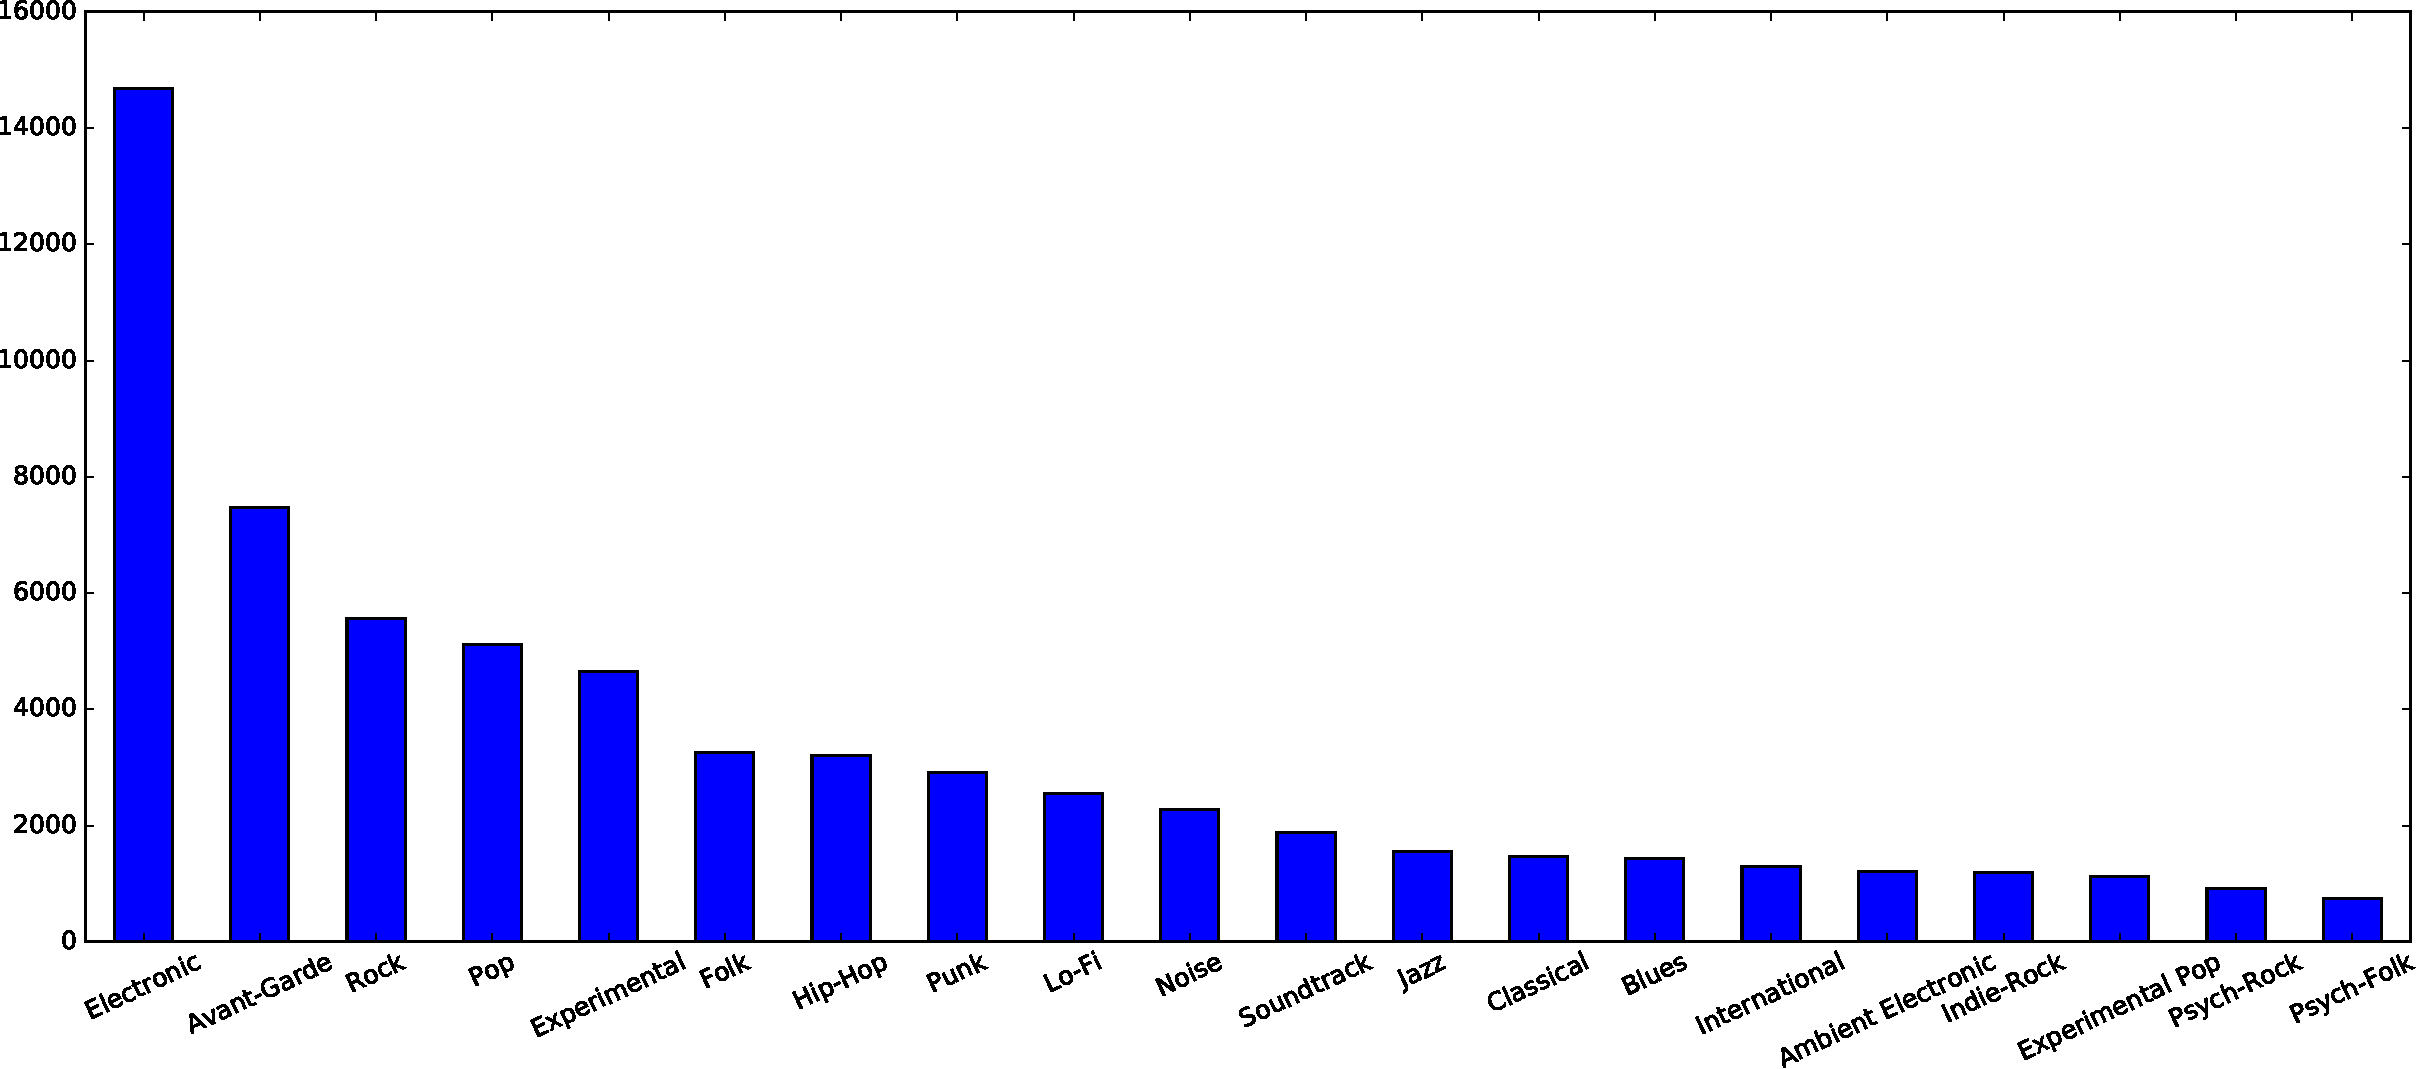
\includegraphics[width=\linewidth]{histo_large.pdf}
	\caption{Power law distribution of the top 20 genres.}
	\label{fig:genres}
\end{figure}

\begin{figure}
	\centering
	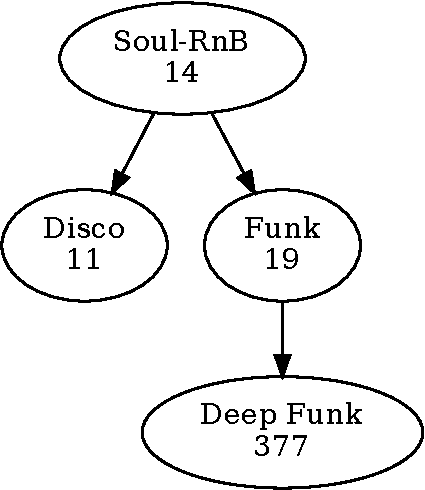
\includegraphics[width=0.5\linewidth]{genre_hierarchy.pdf}
	\caption{Genre hierarchy example from the top-level Soul-RnB genre, \texttt{genre\_id}=14.}
	\label{fig:genre_hierarchy}
\end{figure}

\subsection{Features} % Feature sets

We extracted a wide range of audio features from the audio, using the \href{https://github.com/librosa/librosa}{librosa} Python library. An overview
on these features is given in \tabref{tab:features}.
In addition, a number of descriptive medium-level and high-level audio features extracted by \href{http://the.echonest.com/}{The Echo Nest}, a music platform for developers and media companies, are provided for some tracks. These features include tempo, loudness, timings of fade-in and fade-out, and MFCC-like features for a number of segments.
Those features can be obtained either by uploading the songs to their website, which are then analyzed and sent back to the user, or simply retrieved from their database if the songs are known to them, i.e. they were analyzed before. All of which can be done through an \href{http://developer.echonest.com}{API}. In our case, we only retrieved features from songs which were already in their database.
See \texttt{features.ipynb} for more details.

\begin{table}
	\centering
	\begin{tabular}{llr}
		\toprule
		Feature set & Extractor & Dimensionality \\
		\midrule
		MFCCs \cite{mfcc} & librosa & 26 \\
		MFCCs \cite{mfcc} & librosa & 26 \\
		MFCCs \cite{mfcc} & librosa & 26 \\
		\bottomrule
	\end{tabular}
	\caption{Overview of features extracted from the FMA samples.}
	\label{tab:features}
\end{table}

\subsection{Splits}

A train / test split is proposed to make research on the FMA reproducible.
Below are the constraints we followed:
\begin{enumerate}
	\item For each genre, we randomly split train and test songs with the same ratio 80-20\%.
	\item We forced an artist to be either in the train set, or the test set (meaning the artist's songs cannot be in both train and test sets).
	\item We filled alternatively the train set and test set in the descending order of the count of artist songs. This forces the two sets to have the same distribution of songs per artist.
\end{enumerate}
A track is assigned in train or split for all the subsets and the above constraints are satisfied for all sets. See \texttt{creation.ipynb} for full details.

\subsection{Subsets} \label{sec:subsets}

\begin{table}
	\centering
	\begin{tabular}{lrrccc}
		\toprule
		dataset & clips & genres & length & \multicolumn{2}{c}{Size} \\
		\cmidrule{5-6}
		        &         &          &  [s]   & [GB] & [days] \\
		\midrule
		small  &   4,000 & 10  & 30    & 3.4  & 1.4  \\
		medium &  14,511 & 20  & 30    & 12.2 & 5.1  \\
		large  & 110,000 & 164 & 30    & 90   & 26.9 \\
		full   & 110,000 & 164 & <1800 & 900  & 229  \\
		\bottomrule
	\end{tabular}
	\caption{Proposed subsets of the FMA.}
	\label{tab:subsets}
\end{table}

Finally, for the dataset to be useful as a development set or for people with lower computational resources, we propose the following subsets, each of which is a subset or the larger set:
\begin{enumerate}
	\item \textbf{Full}: this is the complete dataset as described in \secref{sec:content}.
	\item \textbf{Large}: this is the full dataset except audio is 30 seconds clips extracted from the middle of the tracks.
	\item \textbf{Medium}: all tracks which have Echonest features.
	\item \textbf{Small}: tracks from 10 top-level genres, balanced with 400 tracks per genre, 1 genre per track. This subset is similar to the very popular GTZAN in terms of size and genre distribution with the added benefits of the FMA, that is meta-data, pre-computed features and copyright-free audio.
\end{enumerate}
\tabref{tab:subsets} highlights the main differentiating factors between the proposed subsets. See \texttt{analysis.ipynb} for an analysis of the subsets' content similar to that shown in \secref{sec:content}.


%%%%%%%%%%%%%%%%%%%%%%%%%%%%%%%%%%%%%%%%%%%%%%%%%%%%%%%%%%%%%%%%%%%%%%%%%%%%%%%%
\section{Proposed usage} % tasks, usage, problems
%%%%%%%%%%%%%%%%%%%%%%%%%%%%%%%%%%%%%%%%%%%%%%%%%%%%%%%%%%%%%%%%%%%%%%%%%%%%%%%%
% List some MIR tasks and propose some who can be done with that dataset

% MSD: metadata analysis, artist recognition, automatic music tagging, recommendation, cover song recognition, lyrics, limitations

% MSD website typical MIR tasks:
% Segmentation
% Automatic tagging
% Year recognition
% Imputation of missing data
% Artist name, release, song title analysis
% Preview audio
% Yahoo ratings dataset
% Visualization
% Artist recognition
% Cover song recognition
% Lyrics

genre classification, mood classification, artist identification/recognition, instrument recognition, music annotation (tags),
Artist Identification, Genre classification, Mood Classification, Instrument identification, Music Similarity, Autotagging, Automatic playlist generation

Can be down: genre, artist, popularity prediction, tags, year prediction
% Cannot: mood, style, annotations

% Use: unsupervised learning for categorization, does genre emerge how ?
% Task: classify 3secs excerpt. Much more samples, voting is often used.

% TODO
% Problems
% Genre classif / mutli-genre classif
% Recommendation
% Play count prediction
% Covers: generate covers per genre / artist

Meta-data analysis: which genres are artists contributing to, drift in time, curators.
While this collection does obviously not contain hits from well-known artists, it would be interesting to study to what extent it is representative of mainstream music.
%is representative of the commercial music that most users are interested in.

As it happened with e.g. the MSD, people may find and link other sources of data with the dataset, such as lyrics or tags associated to the songs, e.g. from last.fm.

We propose three genre classification problems of varying difficulty.

\begin{enumerate}
	\item Easy, based on \texttt{fma\_small.zip}: 10 top-level genres, balanced with 400 tracks per genre, 1 genre per track
	\item Medium, based on \texttt{fma\_medium.zip}: all 16 top-level genres, unbalanced with x-y tracks per genre, multiple genres per track
	\item Hard, based on \texttt{fma\_large.zip}: all 164 genres, unbalanced with x-y tracks per genre, multiple genres per track
\end{enumerate}

Training / testing division.

\subsection{Limitations}

\todo{what cannot be done currently}

We can however expect people to cross-reference the dataset with other resources to unlock additional tasks, as has happened for example with the MSD and \href{http://www.allmusic.com}{AllMusic}, \href{https://www.last.fm}{last.fm} and \href{https://beatunes.com}{beaTunes} for genre recognition \cite{msd_features, msd_genres}, \href{https://musixmatch.com}{musixmatch} for lyrics, \href{https://secondhandsongs.com}{SecondHandSongs} for cover songs, or \href{https://www.thisismyjam.com}{This Is My Jam} for user play counts.


%%%%%%%%%%%%%%%%%%%%%%%%%%%%%%%%%%%%%%%%%%%%%%%%%%%%%%%%%%%%%%%%%%%%%%%%%%%%%%%%
\section{Genre Recognition} % MGR, Baselines
%%%%%%%%%%%%%%%%%%%%%%%%%%%%%%%%%%%%%%%%%%%%%%%%%%%%%%%%%%%%%%%%%%%%%%%%%%%%%%%%
% One of the most common task, we give some baselines so that people have a reference about how hard it is.
% ground truth for genre: AllMusic Guide (album, artist), Gracenote CDDB (song)

% MSD: Year Prediction

% genre not defined by audio content only
While the utility of music genre recognition (MGR) has been debated, mostly because of its ambiguity and cultural definition, it is widely used and understood by end-users who find it useful to discuss musical categories \cite{mgr_why}. Moreover, it is one of the most researched areas of MIR.

\subsection{Data}

While there certainly is noise in our labels, we trust the artists to have selected the most appropriate set of genres for their own songs.

% Spectrograms of audio data by concatenating 10 spectrograms of 3sec into a single long vector.
% DL on spectrograms
% DL on audio (should work better)

\subsection{Methods}

To assess the difficulty of the task we tested various standard classifiers on mainstream features.

A major motivation to construct the dataset was to apply the powerful Deep Learning techniques to music analysis. As a preliminary result, we trained a convolutional neural network on 3sec-spectrograms, and we select the class by majority voting.

\subsection{Evaluation and results}

The performance of various classifiers on various features are shown in \tabref{tab:mgr} as baselines for future work.
See \texttt{baselines.ipynb} for more details.

%Table xxx reports the classification accuracy on the train and test datasets.\\

\begin{table}
	\centering
	\begin{tabular}{lccccc}
		\toprule
		Features & NB & SVM & kNN & DT & RF \\
		\midrule
		MFCCs  & 30.12 & 30.12 & 30.12 & 30.12 \\
		MFCCs  & 30.12 & 30.12 & 30.12 & 30.12 \\
		MFCCs  & 30.12 & 30.12 & 30.12 & 30.12 \\
		Echonest  & 30.12 & 30.12 & 30.12 & 30.12 \\
		\bottomrule
	\end{tabular}
	\caption{Genre recognition results for various features and classifiers.}
	\label{tab:mgr}
\end{table}


%%%%%%%%%%%%%%%%%%%%%%%%%%%%%%%%%%%%%%%%%%%%%%%%%%%%%%%%%%%%%%%%%%%%%%%%%%%%%%%%
\section{Conclusion and Perspectives}
%%%%%%%%%%%%%%%%%%%%%%%%%%%%%%%%%%%%%%%%%%%%%%%%%%%%%%%%%%%%%%%%%%%%%%%%%%%%%%%%
% MSD: the future of the dataset, visibility for MIR (to DL people!)

% importance of open data

Content-based music information retrieval tasks are typically solved with a two-stage approach: engineered features are extracted from music audio signals, and are then used as input to a regressor or classifier.
Although that approach was dominant in the past, feature learning and end-to-end learning (from signal to label) have started to receive more attention from the MIR community in recent years. 
The primary goal of this dataset is to enable researchers to train large models, which require lots of training data, which could potentially avert the semantic gap currently observed between the extracted low-level features such as MFCCs and the high-level targets such as genre.
Hopefully, the release of such amount of easily accessible data will foster research which will ultimately surpass the performance ceiling observed in e.g. genre recognition, as it as been the case in computer vision with the release of ImageNet.

The FMA enables researchers to test algorithms on a large-scale collection, thus allowing to test them on more real-world like environments. By providing audio, we do not limit the benchmarking to pre-computed features and allow scientists to develop and test new feature sets, learn features, or learn mappings directly from the audio.
While MGR has been MIR's flagship application for a while, prediction accuracy reached a glass ceiling \cite{mgr_why}. We hope that the advent of a massive open dataset for that task will have the same effect as the release of ImageNet, i.e. a massive improvement in accuracy thanks to the advent of specialized deep learning architectures with testable performances which can be compared.
Thanks to the availability of audio, deep learning architectures such as convolutional neural networks and recurrent neural networks can be directly applied to the waveform, bypassing any feature engineering. Such exploration may hopefully provide alternatives to solving MIR challenges \cite{mir_dl_feature_learning}.
However, while this release is pretty large, we shall keep in mind that it is still two orders of magnitude behind commercial services who have access to tens of millions of songs.\footnote{\href{http://the.echonest.com}{37M Echonest}, \href{https://en.wikipedia.org/wiki/Spotify}{30M Spotify}, \href{http://www.skilledtests.com/wiki/Last.fm_statistics}{45M last.fm}, \href{http://bupz.com/best-websites-to-buy-musics}{45M 7digital}, \href{https://www.apple.com/pr/library/2013/02/06iTunes-Store-Sets-New-Record-with-25-Billion-Songs-Sold.html}{26M iTunes}}

% Once that problem is well advanced, researchers will be able to tackle more difficult tasks such as tagging or annotation.
% Besides, standard data analysis tasks such as classification, clustering, regression, text analysis, visualization can also be applied to this new music dataset.


%%%%%%%%%%%%%%%%%%%%%%%%%%%%%%%%%%%%%%%%%%%%%%%%%%%%%%%%%%%%%%%%%%%%%%%%%%%%%%%%
\section{Acknowledgments}
%%%%%%%%%%%%%%%%%%%%%%%%%%%%%%%%%%%%%%%%%%%%%%%%%%%%%%%%%%%%%%%%%%%%%%%%%%%%%%%%


We are grateful to SWITCH and EPFL for hosting the dataset within the context
of the \href{https://projects.switch.ch/scale-up}{SCALE-UP} project, funded in
part by the swissuniversities \href{http://www.swissuniversities.ch/isci}{SUC
P-2 program}.

We are grateful to the team supporting the \href{https://freemusicarchive.org}{Free Music Archive} as well as all the contributing artists and curators for the fantastic content they made available.

We also want to thank the team behind \href{https://zenodo.org}{zenodo.org}, whose free hosting and archiving of digital research artifacts is promoting a more open scientific process.

\bibliography{refs}
\end{document}
